%%%%%%%%%%%%%%%%%%%%%%%%%%%%%%%%%%%%%%%%%
% Short Sectioned Assignment
% LaTeX Template
% Version 1.0 (5/5/12)
%
% This template has been downloaded from:
% http://www.LaTeXTemplates.com
%
% Original author:
% Frits Wenneker (http://www.howtotex.com)
%
% License:
% CC BY-NC-SA 3.0 (http://creativecommons.org/licenses/by-nc-sa/3.0/)
%
%%%%%%%%%%%%%%%%%%%%%%%%%%%%%%%%%%%%%%%%%

%----------------------------------------------------------------------------------------
%	PACKAGES AND OTHER DOCUMENT CONFIGURATIONS
%----------------------------------------------------------------------------------------

\documentclass[paper=a4, fontsize=11pt]{scrartcl} % A4 paper and 11pt font size

\usepackage[T1]{fontenc} % Use 8-bit encoding that has 256 glyphs
\usepackage{fourier} % Use the Adobe Utopia font for the document - comment this line to return to the LaTeX default
\usepackage[english]{babel} % English language/hyphenation
\usepackage{amsmath,amsfonts,amsthm, amssymb} % Math packages
\usepackage{enumitem}
\usepackage{cancel}
\usepackage{graphicx} % Required to insert images
\usepackage{color}
\definecolor{dkgreen}{rgb}{0,0.6,0}
\definecolor{gray}{rgb}{0.5,0.5,0.5}
\definecolor{mauve}{rgb}{0.58,0,0.82}
\usepackage{listings}
\lstset{frame=tb,
  language=Python,
  aboveskip=3mm,
  belowskip=3mm,
  showstringspaces=false,
  columns=flexible,
  basicstyle={\small\ttfamily},
  numbers=none,
  numberstyle=\tiny\color{gray},
  keywordstyle=\color{blue},
  commentstyle=\color{dkgreen},
  stringstyle=\color{mauve},
  breaklines=true,
  breakatwhitespace=true
  tabsize=3
}
\usepackage{pgfplotstable}% For inserting csv table

\usepackage{sectsty} % Allows customizing section commands
\allsectionsfont{\centering \normalfont\scshape} % Make all sections centered, the default font and small caps

\usepackage{fancyhdr} % Custom headers and footers
\pagestyle{fancyplain} % Makes all pages in the document conform to the custom headers and footers
\fancyhead{} % No page header - if you want one, create it in the same way as the footers below
\fancyfoot[L]{} % Empty left footer
\fancyfoot[C]{} % Empty center footer
\fancyfoot[R]{\thepage} % Page numbering for right footer
\renewcommand{\headrulewidth}{0pt} % Remove header underlines
\renewcommand{\footrulewidth}{0pt} % Remove footer underlines
\setlength{\headheight}{13.6pt} % Customize the height of the header

\numberwithin{equation}{section} % Number equations within sections (i.e. 1.1, 1.2, 2.1, 2.2 instead of 1, 2, 3, 4)
\numberwithin{figure}{section} % Number figures within sections (i.e. 1.1, 1.2, 2.1, 2.2 instead of 1, 2, 3, 4)
\numberwithin{table}{section} % Number tables within sections (i.e. 1.1, 1.2, 2.1, 2.2 instead of 1, 2, 3, 4)

\setlength\parindent{0pt} % Removes all indentation from paragraphs - comment this line for an assignment with lots of text

%----------------------------------------------------------------------------------------
%	TITLE SECTION
%----------------------------------------------------------------------------------------

\newcommand{\horrule}[1]{\rule{\linewidth}{#1}} % Create horizontal rule command with 1 argument of height

\title{	
\normalfont \normalsize 
\textsc{Baruch, MFE} \\ [25pt] % Your university, school and/or department name(s)
\horrule{0.5pt} \\[0.4cm] % Thin top horizontal rule
\huge MTH 9876 Assignment Three\\  % The assignment title
\horrule{2pt} \\[0.5cm] % Thick bottom horizontal rule
}


\author{Zhou, ShengQuan} % Your name

\date{\normalsize\today} % Today's date or a custom date

\begin{document}
	


\maketitle % Print the title

\newpage



\section{Bootstrapping of Survival Curves}
The enclosed spreadsheet contains a snapshot of actual par spreads (as of October 6, 2015) of several
names: General Electric, JPMorgan Chase, Axis Capital, and MBIA. The values of the spreads are
expressed in basis points (i.e., the value of 45 means 0.0045). In the calculations below, assume that
the recovery rate is 40\%, and the riskless rate $r$ is constant and equal $1.5\%$.
\begin{center}
\begin{tabular}{l*{6}{r}r}
Name              & 1Y & 2Y & 3Y & 4Y & 5Y  & 7Y & 10Y \\
\hline
GE	& 19.35	& 25.45 &	31.85	& 38	& 47.9	& 71	& 93.6\\
JPM	& 38.8	& 51.5	& 61.45	& 72.5	& 89.6	& 111.05	& 131.7\\
Axis &	152.5	& 200.75	& 235.75	& 241.3	& 264.2	& 269.8	& 272.05\\
MBIA &	393.35	& 463.2	& 563.25	& 696.4	& 727.2	& 749.4	& 735.5\\
\end{tabular}
\end{center}

\textbf{(i)} Use the valuation formulas and the bootstrap method explained in Lecture 3 to build the survival curves
for each of these names.\\
\textit{Solution}: According to Lecture 3, the protection leg
\begin{align*}
V_{\text{prot}}(T_i) &= -(1-R)\int_0^T P(0,s)dS(0,s)\approx \frac{1-R}{2}\sum_{j=1}^{n_i} \left[ P(0,s_{j-1}) + P(0,s_j) \right]
\left[ S(0,s_{j-1}) - S(0,s_j) \right],
\end{align*}
where $S(0,t)=e^{-t\bar{\lambda}(t)}$, $P(0,t)=e^{-rt}$, and $n_i$ is the number discretized time steps up to $T_i$. In practice, it is sufficient to choose the time steps monthly for sufficient accuracy.
Assume that  we have $K$ CDSs with maturities $T_1<T_2<\cdots T_K$. In the simplest approach, we assume that $\bar{\lambda}(t)$ is piecewise constant
between the times $T_i, i=1,2,\cdots,K$. Let $\bar{\lambda}_i$ be the constant forward intensity on the interval $[T_{i-1},T_i]$, where $T_0=0$. On the other hand,
according to the approximation given in Lecture 3, the risky annuity of premium leg
\begin{align*}
\mathcal{A}(T_i) &= \frac{\delta}{2}\sum_{j=1}^{N_i} P(0,t_j)\left[ S(0,t_{j-1}) + S(0,t_j) \right],
\end{align*}
where $N_i$ is the number of quarterly roll dates $t_j$ up to $T_i$ (not including $T_0$) and $\delta = \frac{1}{4}$. The par credit spread observed 
from market is
$$
C_0(T_i) = \frac{V_{\text{prot}}(T_i)}{\mathcal{A}(T_i)}.
$$
More explicitly,
\begin{equation}\label{spread}
C_0(T_i) = \left(\frac{1-R}{\delta}\right)\cdot\frac{\sum_{j=1}^{n_i} \left[ e^{-rs_{j-1}} + e^{-rs_j} \right]\left[ e^{-\bar{\lambda}(s_{j-1})s_{j-1}} - e^{-\bar{\lambda}(s_{j})s_{j}} \right]}
{ \sum_{j=1}^{N_i} e^{-rt_j}\left[e^{-\bar{\lambda}(t_{j-1})t_{j-1}} + e^{-\bar{\lambda}(t_{j})t_{j}} \right]},\quad i=1,2,3,4,5,7,10.
\end{equation}

In this exercise, we choose $s_0=t_0=0$, $s_{j}-s_{j-1}=\frac{1}{12}$, $t_{j}-t_{j-1}=\delta=\frac{1}{4}$, $R=0.4$, and $r=1.5\%$. The survival curves
are plotted in Fig. \ref{survival}. For Axis and MBIA, zig-zag patterns are observed in the survival curve which violates the no-arbitrage condition
$\frac{dS(0,t)}{dt}\le 0$.
\begin{figure}[h]\label{survival}
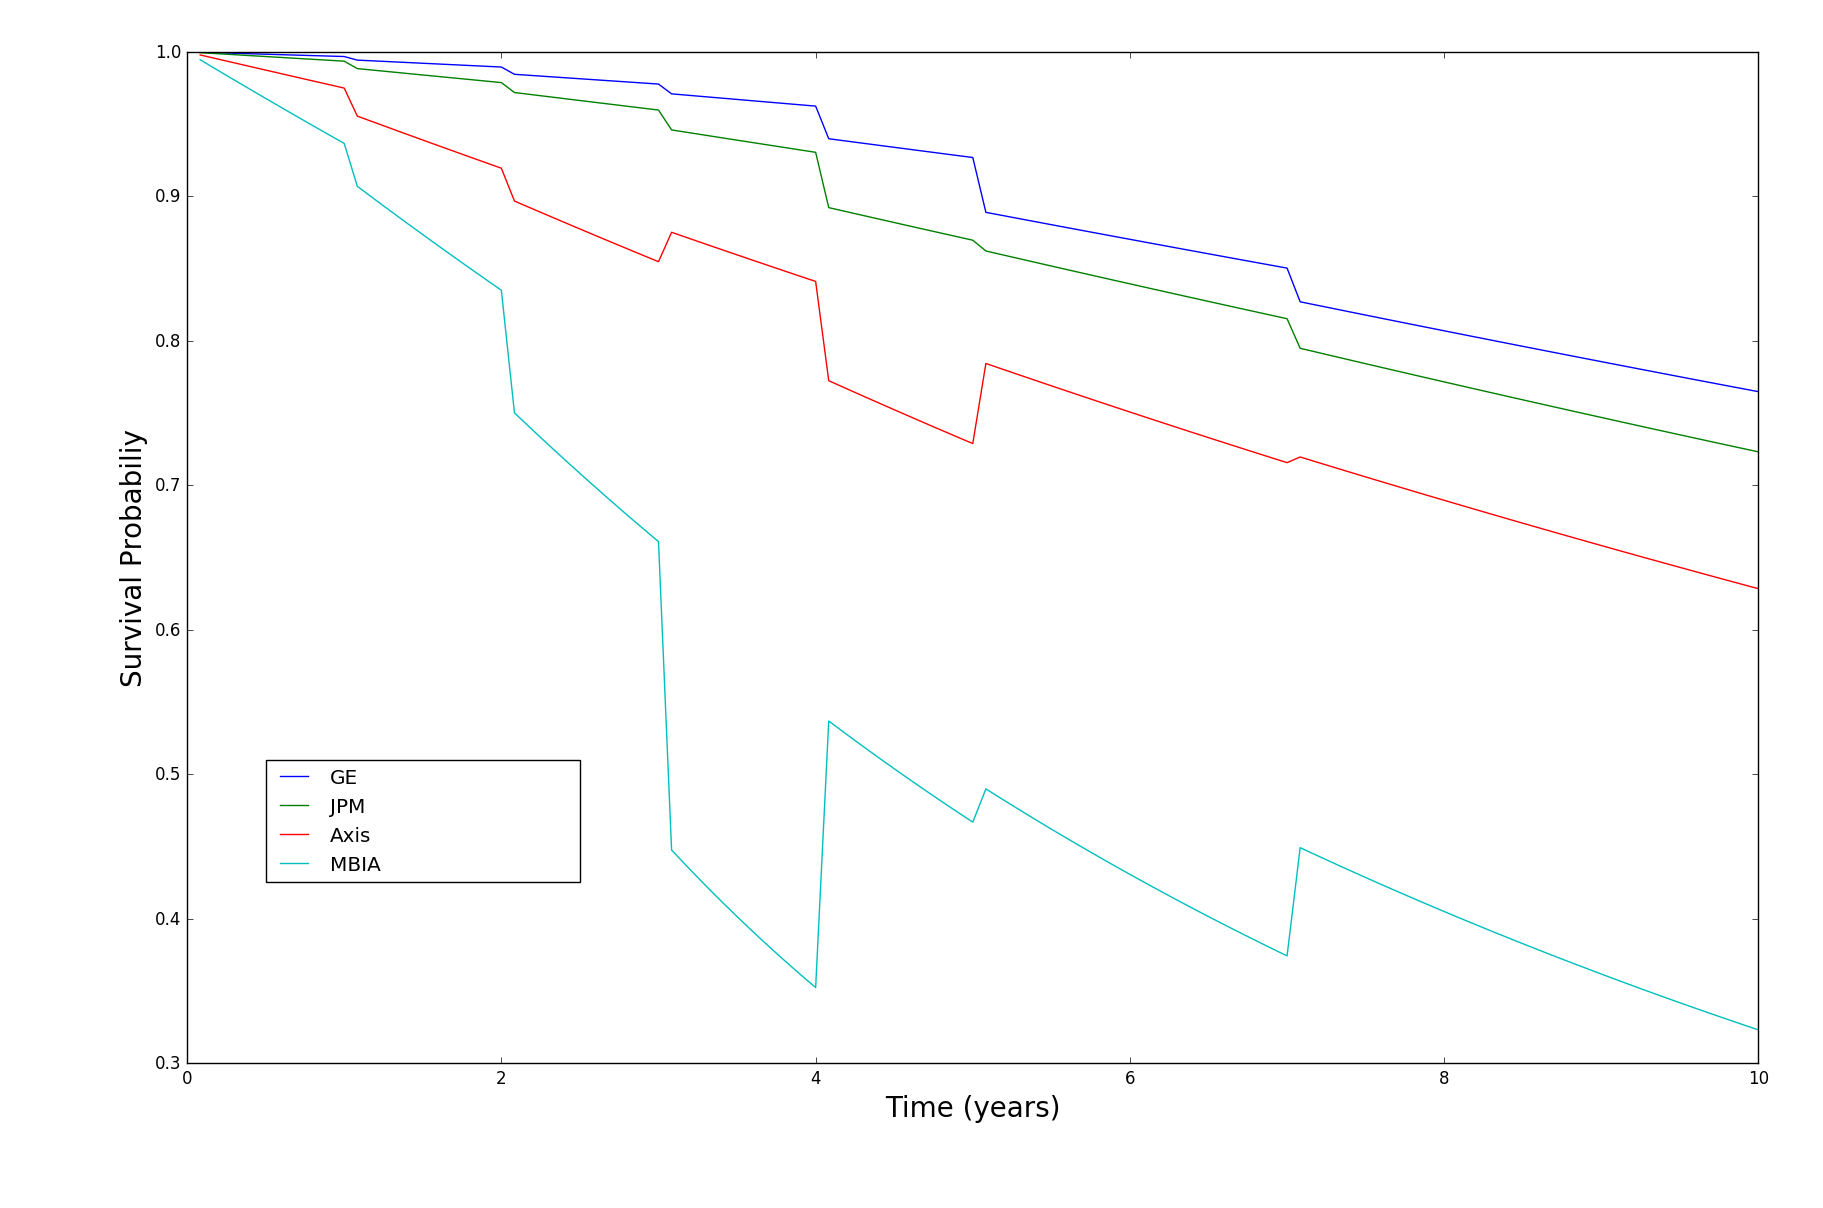
\includegraphics[width=15cm]{survival_curve}
\end{figure}

\newpage
\textbf{(ii)} Based on these curves, calculate the default probabilities of each of these names in $T=1,2,\cdots, 10$
years.\\
\textit{Solution}: The default probabilities in $T=1,2,\cdots, 10$ are tabulated in the following:
\begin{center}
\pgfplotstabletypeset[
    col sep=comma,
    string type,
    columns/natural/.style={column name=natural, column type={|l}},
    columns/two/.style={column name=two, column type={|l}},
    columns/three/.style={column name=three, column type={|c|}},
    every head row/.style={before row=\hline,after row=\hline},
    every last row/.style={after row=\hline},
    ]{default.csv}
\end{center}


\textbf{(iii)} For each of these names, compute the par spread for the 2Y into 5Y forward CDS.\\
\textit{Solution}: For some conventions in forward starting instruments, refer to MTH9878 \textit{Interest Rate Models} Lecture 3, Page 75, 78. The 
par spread of a forward CDS is given by a similar formula as Eq.\ref{spread} with the summation restricted to the time window 2Y$\rightarrow$7Y, tabulated
as follows:
\begin{center}
\begin{tabular}{l*{6}{c}r}
\hline
Name              & GE & JPM & Axis & MBIA  \\
\hline
Par Spread (bps)	& 63.99	& 117.70 &	315.14	& 1039.01\\
\hline
\end{tabular}
\end{center}

Python script:
\begin{lstlisting}
import math
import numpy as np
from scipy.optimize import fsolve
import matplotlib.pyplot as plt

f, axarr = plt.subplots(1)

# input parameters
R = 0.4 # recovery rate
r = 0.015 # riskless interest rate
timeStepsPerYear = 12
rollDatesPerYear = 4

# constants
bps = 0.0001

# derived paramters
rollDatesInterval = int(timeStepsPerYear/rollDatesPerYear)
delta = 1.0/rollDatesPerYear # interval between roll dates
dt = 1.0/timeStepsPerYear # time step width for Stieltjes integral
c = (1-R)/delta
numOfMaturities = len(CdsMaturities)
maxMaturity = CdsMaturities[numOfMaturities-1]
maxNumOfTimeSteps = maxMaturity*timeStepsPerYear

def CalcParSpread(x, minUnknownIndex, maxUnknownIndex, knownIntensities):
    numerator = 0.0
    denominator = 0.0
    for i in range(maxUnknownIndex):
        l = 0.0
        if i >= minUnknownIndex: l = x
        else: l = knownIntensities[i]

        P = math.exp(-r*i*dt) + math.exp(-r*(i+1)*dt)
        S = math.exp(-l*i*dt) - math.exp(-l*(i+1)*dt)
        numerator += P*S
        
    for i in range(0,maxUnknownIndex,rollDatesInterval):
        l = 0.0
        if i >= minUnknownIndex: l = x
        else: l = knownIntensities[i]

        P = math.exp(-r*(i+rollDatesInterval)*dt)
        S = math.exp(-l*i*dt) + math.exp(-l*(i+rollDatesInterval)*dt)
        denominator += P*S
        
    return c*numerator/denominator

def func(x, *data):
    return CalcParSpread(x, data[0], data[1], data[2])-data[3]

def CalcIntensity(parSpreads, knownIntensities):
    minUnknownIndex = None
    maxUnknownIndex = None
    currentParSpread = None
    for i in range(numOfMaturities):
        currentParSpread = parSpreads[i]
        minUnknownIndex = 0
        if i>0: minUnknownIndex = CdsMaturities[i-1]*timeStepsPerYear
        maxUnknownIndex = CdsMaturities[i]*timeStepsPerYear

        lambda0 = currentParSpread/(1-R)
        data = (minUnknownIndex, maxUnknownIndex, knownIntensities, currentParSpread)
        y = fsolve(func, lambda0, args=data)
        for j in range(minUnknownIndex,maxUnknownIndex):
            knownIntensities[j] = y[0]

    survivalRates = []
    for i in range(maxNumOfTimeSteps):
        survivalRates.append(math.exp(-(i+1)*dt*knownIntensities[i]))
  
    return survivalRates

timeAxis = []
for i in range(maxNumOfTimeSteps):
    timeAxis.append((i+1)*dt)

CdsParSpreads = np.array([19.35,25.45,31.85,38.0,47.9,71.0,93.6])*bps
knownIntensities = [None]*maxNumOfTimeSteps
survivalRates = CalcIntensity(CdsParSpreads, knownIntensities)
axarr.plot(timeAxis, survivalRates, label="GE")
\end{lstlisting}

\newpage

\section{Andersen's Method for Pricing a Single Period CMDS}
Consider Anderson's method for pricing a single period CMDS as discussed in class.
Let $\alpha$ be te participation rate (known). Assume  the underlying spread is
lognormally distributed,
$$
\varphi(x) = \frac{1}{\sqrt{2\pi \sigma^2 T_{i-1}}x} \exp\left(
-\frac{\left( \log\left(\frac{x}{C_0}\right) + \frac{1}{2}\sigma^2 T_{i-1} \right)^2}{2\sigma^2 T_{i-1}}
\right)
$$
The price of a CMDS is often quoted in terms of a \textit{participation rate}. This is the factor which
we use to multiply all of the coupons on the CMDS so that their present value equals the present value
of the protection leg.\\
\textbf{(i)} Calculate $V_{\text{cpn}}(0)$ assuming no cap on the spread.\\
\textit{Solution}: The example given in Lecture 4 is concerned with the case of 
\begin{itemize}[noitemsep]
\item Settlement date $T_0$, CMDS coupon payment date $T_1$;
\item $C(T_0)\triangleq C(T_0,T_0,T)$: par spread of the reference swap $T_0\rightarrow T$, known at $T_0$;
\item Under survival measure, $\mathbb{E}^{\mathbb{Q}_{T_0,T}}[C(T_0,T_0,T)] = C(0,T_0,T)\triangleq C_0$, known at time zero;
\item Approximation of $f(C)\approx aC+b$, where
$$
b = \frac{P_0(T_1)}{A_0(T_0,T)}, \quad
a = \frac{1}{C_0}\left(\frac{\mathcal{P}_0(T_1)}{\mathcal{A}_0(T_0,T)}-b\right) = \frac{1 }{C_0}\left(\frac{\mathcal{P}_0(T_1)}{\mathcal{A}_0(T_0,T)}- \frac{P_0(T_1)}{A_0(T_0,T)}\right).
$$
\end{itemize}
In this exercise, denote the constant maturity $\Delta T = T-T_0$, the above parameters are adjusted accordingly
\begin{itemize}[noitemsep]
\item Settlement date $T_{i-1}$, CMDS coupon payment date $T_i$;
\item $C_0\triangleq C(0,T_{i-1},T_{i-1}+\Delta T)$: par spread of the reference swap $T_{i-1}\rightarrow T_{i-1}+\Delta T$, valuated at time zero. The survival measure is $\mathbb{Q}_{T_{i-1},T_{i-1}+\Delta T}$.
\item Approximation of $f(C)\approx aC+b$, where
\begin{align*}
b &= \frac{P_0(T_i)}{A_0(T_{i-1}, T_{i-1}+\Delta T)},\\
a &= \frac{1}{C_0}\left(\frac{\mathcal{P}_0(T_i)}{\mathcal{A}_0(T_{i-1}, T_{i-1}+\Delta T)}-b\right) = \frac{1 }{C_0}\left(
\frac{\mathcal{P}_0(T_i)}{\mathcal{A}_0(T_{i-1}, T_{i-1}+\Delta T)}- \frac{P_0(T_i)}{A_0(T_{i-1}, T_{i-1}+\Delta T)}\right).
\end{align*}
\end{itemize}
Now invoking Anderson's result:
\begin{align*}
V_{\text{cpn}}(0) &= \mathcal{A}(0)\delta \mathbb{E}^{\mathbb{Q}_{T_{i-1},T_{i-1}+\Delta T}}\left[f(C)C\right]\\
 &\approx \mathcal{A}(0)\delta \mathbb{E}^{\mathbb{Q}_{T_{i-1},T_{i-1}+\Delta T}}\left[aC^2+bC\right]\\
 &= \mathcal{A}(0)\delta \left(a\mathbb{E}^{\mathbb{Q}_{T_{i-1},T_{i-1}+\Delta T}}\left[C^2\right]+b\mathbb{E}^{\mathbb{Q}_{T_{i-1},T_{i-1}+\Delta T}}\left[C\right]\right)\\
 &= \mathcal{A}(0)\delta \left(a e^{2\log C_0-\sigma^2 T_{i-1}+ 2\sigma^2 T_{i-1}} + b e^{\log C_0 - \frac{1}{2}\sigma^2 T_{i-1} + \frac{1}{2}\sigma^2 T_{i-1}}\right)\\
  &= \mathcal{A}(0)\delta \left(a C_0^2e^{\sigma^2 T_{i-1}} + b C_0\right),
\end{align*}
where $\mathcal{A}(0)\triangleq \mathcal{A}(0,T_{i-1},T_{i-1}+\Delta T)$, and we have used the well-known results on the first two moments of a lognormal variable: $\mathbb{E}[X]=e^{\mu + \frac{1}{2}\sigma^2}$, and $\mathbb{E}[X^2]=e^{2\mu+2\sigma^2}$.\\


\textbf{(ii)} Calculate $V_{\text{cpn}}(0)$ assuming a cap of $U$ on the spread.\\
\textit{Solution}: Under Anderson's method,
\begin{align*}
V_{\text{cpn}}(0) &= \alpha \mathcal{A}(0)\delta \int_0^{\infty} (ax+b)\min(x,U)\varphi(x)dx\\
&= \alpha \mathcal{A}(0)\delta \left[ \int_0^{U} (ax^2+bx)\varphi(x)dx
+  U \int_U^{\infty} (ax+b)\varphi(x)dx \right].
\end{align*}
Since $\varphi(x)$ is a lognormal distribution, let $y=\log x$ and $y$ is normally distributed
\begin{align*}
\varphi(x)dx &= \frac{1}{\sqrt{2\pi \sigma^2 T_{i-1}}x} \exp\left(
-\frac{\left( \log\left(\frac{x}{C_0}\right) + \frac{1}{2}\sigma^2 T_{i-1} \right)}{2\sigma^2 T_{i-1}}
\right) dx\\
 &= \frac{1}{\sqrt{2\pi \sigma^2 T_{i-1}}} \exp\left(
-\frac{\left( y -\log C_0 + \frac{1}{2}\sigma^2 T_{i-1} \right)^2}{2\sigma^2 T_{i-1}}
\right) dy\\
&\triangleq \phi(y)dy,
\end{align*}
with mean $\mu = \log C_0 -  \frac{1}{2}\sigma^2 T_{i-1}$ and variance $s^2 = \sigma^2 T_{i-1}$. Thus,
$$
V_{\text{cpn}}(0)
 = \alpha \mathcal{A}(0)\delta \left[\int_{-\infty}^{\log U} (ae^{2y}+be^y)\phi(y)dy
+  U \int_{\log U}^{\infty} (ae^y +b)\phi(y)dy\right].
$$
In general, for any $d,u,\beta\in\mathbb{R}$,
\begin{align*}
\int_d^u e^{\beta y}\phi(y)dy &= \frac{1}{\sqrt{2\pi}s}\int_d^u e^{-\frac{(y-\mu)^2}{2s^2}+\beta y}dy \\
&= \frac{e^{ \beta \mu +\frac{1}{2}s^2\beta^2}}{\sqrt{2\pi}s}\int_d^u e^{-\frac{(y-\mu - s^2\beta)^2}{2s^2}}dy \\
&= e^{ \beta \mu +\frac{1}{2}s^2\beta^2} \int_{\frac{d-\mu -s^2\beta}{s}}^{\frac{u-\mu - s^2\beta}{s}} \frac{1}{\sqrt{2\pi}}e^{-\frac{y^2}{2}}dy \\
& = e^{ \beta \mu +\frac{1}{2}s^2\beta^2} \left[ N\left(\frac{u-\mu - s^2\beta}{s} \right) -  N\left(\frac{d-\mu - s^2\beta}{s}\right) \right].
\end{align*}
Specifically,
\begin{align*}
a\int_{-\infty}^{\log U} e^{2y}\phi(y)dy &=a C_0^2 e^{\sigma^2 T_{i-1}} N\left(\frac{\log\frac{U}{C_0}-  \frac{3}{2}\sigma^2 T_{i-1}}{\sigma\sqrt{T_{i-1}}} \right),\\
b\int_{-\infty}^{\log U} e^{y}\phi(y)dy &=b C_0 N\left(\frac{\log\frac{U}{C_0}-  \frac{1}{2}\sigma^2 T_{i-1}}{\sigma\sqrt{T_{i-1}}} \right),\\
Ua \int_{\log U}^{\infty} e^{y}\phi(y)dy &= Ua C_0N\left(-\frac{\log\frac{U}{C_0}-  \frac{1}{2}\sigma^2 T_{i-1}}{\sigma\sqrt{T_{i-1}}} \right),\\
Ub \int_{\log U}^{\infty} \phi(y)dy &= Ub N\left(-\frac{\log\frac{U}{C_0}+  \frac{1}{2}\sigma^2 T_{i-1}}{\sigma\sqrt{T_{i-1}}} \right).
\end{align*}
Finally,
\begin{align*}
V_{\text{cpn}}(0) = \alpha \mathcal{A}(0)\delta \Bigg[
&a C_0^2 e^{\sigma^2 T_{i-1}} N\left(\frac{\log\frac{U}{C_0}-  \frac{3}{2}\sigma^2 T_{i-1}}{\sigma\sqrt{T_{i-1}}} \right)
+ b C_0 N\left(\frac{\log\frac{U}{C_0}-  \frac{1}{2}\sigma^2 T_{i-1}}{\sigma\sqrt{T_{i-1}}} \right)\\
&+  Ua C_0N\left(-\frac{\log\frac{U}{C_0}-  \frac{1}{2}\sigma^2 T_{i-1}}{\sigma\sqrt{T_{i-1}}} \right) + Ub N\left(-\frac{\log\frac{U}{C_0}+  \frac{1}{2}\sigma^2 T_{i-1}}{\sigma\sqrt{T_{i-1}}} \right)\Bigg].
\end{align*}\\

\textbf{(iii)} What is the value of the cap option?\\
\textit{Solution}: Notice that the payoff of a cap option $(x-U)^+ = x-\min(x,U)$, we can write the value of the cap option as
$
V^{\textbf{(i)}}_{\text{cpn}}(0)-V^{\textbf{(ii)}}_{\text{cpn}}(0)
$, in other words, the difference between the premium legs obtained from part \textbf{(i)} and \textbf{(ii)}.

\newpage

\section{CIR Model of Stochastic Intensity}
Consider the CIR model of stochastic intensity
$$
d\lambda(t) = \kappa(t)(\theta(t) - \lambda(t))dt + \sigma(t)\sqrt{\lambda(t)}dW(t).
$$
Show, by a direct calculation, that the survival probability is of the form
$$
S(t,T) = e^{A(t,T)-C(t,T)\lambda(t)},
$$
where the coefficients $A(t,T)$ and $C(t,T)$ satisfies Riccati's ordinary differential equations
\begin{align*}
& \frac{dA(t)}{dt} -\kappa(t)\theta(t)C(t) = 0,\\
& \frac{dC(t)}{dt} -\kappa(t)C(t) -\frac{1}{2}\sigma^2(t)C^2(t) + 1 = 0,
\end{align*}
subject to the terminal condition $C(T,T) = A(T,T) = 0$.\\
\textit{Solution}: This problem falls into the general category of finding the PDE satisfied by
some expression given a stochastic representation of the expression. The key is to find a martingale. Here we have
\begin{align*}
S(t,T) &= \mathbb{E}\bigg[ e^{-\int_t^T \lambda(t') dt'}  \bigg|\mathcal{G}_t \bigg] = \mathbb{E}\bigg[ e^{\int_0^t  \lambda(t') dt'  - \int_0^T  \lambda(t') dt'}  \bigg|\mathcal{G}_t \bigg]= e^{\int_0^t  \lambda(t') dt' } \mathbb{E}\bigg[ e^{ - \int_0^T  \lambda(t') dt'}  \bigg|\mathcal{G}_t \bigg].
\end{align*}
Thus, using the fact that $S(T,T)=1$,
$$
e^{ -\int_0^t  \lambda(t') dt' }S(t,T) = \mathbb{E}\bigg[ e^{ - \int_0^T  \lambda(t') dt'}  S(T,T)\bigg|\mathcal{G}_t \bigg],
$$
we conclude $e^{ -\int_0^t  \lambda(t') dt' }S(t,T) = e^{ -\int_0^t  \lambda(t') dt' +A(t,T)-C(t,T)\lambda(t) }
\triangleq e^{X(t)}$ is a martingale, where $X(t)=-\int_0^t  \lambda(t') dt' +A(t,T)-C(t,T)\lambda(t)$. Apply It\^o's lemma,
\begin{align*}
& d e^{X(t)} \\
&= e^{X(t)}\left[dX(t)+\frac{1}{2}dX(t)dX(t)\right]\\
&= e^{X(t)}\Bigg[-\lambda(t) dt + A'(t,T)dt -C'(t,T)\lambda(t) dt  \\
&\quad \quad\quad\quad-C(t,T)\left(\kappa(t)\left(\theta(t)- \lambda(t)\right)dt + \sigma(t)\sqrt{\lambda(t)}dW(t)\right) + \frac{1}{2}C^2(t,T)\sigma^2(t)\lambda(t)dt \Bigg]\\
&=e^{X(t)}\left[ \left(-\lambda(t)+ A'(t,T)-C'(t,T)\lambda(t) -C(t,T)\kappa(t)\left(\theta(t)- \lambda(t)\right)+ \frac{1}{2}C^2(t,T)\sigma^2(t)\lambda(t)\right)
dt + \left(\cdots\right)dW(t)\right] \\
&=e^{X(t)}\left[  \left(\boxed{A'(t,T) -C(t,T)\kappa(t)\theta(t)}-\lambda(t)\times\boxed{ 1+ C'(t,T) -C(t,T) \kappa(t)- \frac{1}{2}C^2(t,T)\sigma^2(t)}\right)
dt + \left(\cdots\right)dW(t)\right] .
\end{align*}
Because $e^{X(t)}$ is a martingale, set the drift terms in boxes to zero, we get 
\begin{align*}
&\frac{dA(t)}{dt} - C(t,T)\kappa(t)\theta(t) =0,\\
&\frac{dC(t)}{dt}  -\kappa(t)C(t,T) - \frac{1}{2}\sigma^2(t)C^2(t,T)+1 = 0.
\end{align*}

\end{document}